\scanpage{20}
$\mathrm{Pol}\ \mathrm{top}\longrightarrow\mathrm{Pol}\ \mathrm{comb}$ ess.$^{\mathrm t}$ surjectif : \unsure{dém. abstraite|dim. abstraite}

\uline{Foncteur réalisation topologique}

dualité : échange de $S$ et $A$

\figure{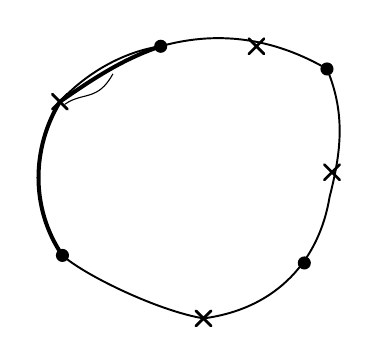
\begin{tikzpicture}[x=0.032cm,y=-0.032cm,line cap=round,line join=round]
\draw[line width=.7pt] (12,30) .. controls (23,18) and (38,10) .. (52,8)
 .. controls (77,1) and (99,6) .. (118,17)
 .. controls (126,36) and (123,52) .. (119,68)
 .. controls (115,92) and (99,112) .. (69,116)
 .. controls (51,113) and (22,99) .. (13,91)
 .. controls (1,73) and (0,50) .. (12,30);
\draw[line width=1.45pt] (13,91) .. controls (0,72) and (1,48) .. (12,30)
 .. controls (25,21) and (37,13) .. (52,8);
\draw (14,31) .. controls (21,26) and (27,30) .. (33,19);
\foreach \x/\y in {52/8,118/17,109/94,13/91}{\fill (\x,\y) circle[radius=2.6];}
\foreach \x/\y in {12/30,90/8,120/58,69/116}{
\draw[line width=1pt] (\x-3,\y-3)--(\x+3,\y+3) (\x-3,\y+3)--(\x+3,\y-3);}
\end{tikzpicture}}

point de vue ens. ordonnés \quad $P=S\amalg A$

\deleted{\unsure{dont}} ($S$ él. minimaux, $A$ éléments maximaux

chaque élément minimal \unsure{majorant|majoré}

chaque élément minimal majoré \inserted{\unsure{str.$^{\mathrm t}$|strt|strict.}} par \unsure{exactemt|exactement} deux él. \unsure{dist.|div.|distincts} maximaux)

chaque élément maximal minoré par exactement deux éléments \unsure{combi.|comb.} minimaux)

ici dualité : renversement de la relation d'ordre

Composantes connexes \deleted{\unsure{des}} \unsure{sont|v$^{\mathrm t}$|v.t.} des \unsure{cercles|ens|ens.} comb.

\deleted{point de vue} polygone combin. (trois définitions comb. équiv.)

Point de vue \uline{ens. de base $S$} (valable si les comp. connexes sont \uline{d'ordre $\geq3$})

$A\hookrightarrow\unsure{\mathfrak P|\mathcal P|P}_2(S)$ structure ens. de parties à deux éléments de $S$ (appelées \uline{arêtes}) tel que $\forall\ s\in S$ appartient à exactemt deux arêtes

Point de vue dual : structure sur $A$, d'un ens $S\hookrightarrow\mathfrak P_2(A)$ (qu'on appellera les ``sommets'')

Point de vue ordres circulaires (cas des polygônes d'ordre $\geq3$) : donnée sur $S$ (ou $A$) d'une paire d'ordres circulaires \inserted{(i.e. permutations transitives)} inverses l'un de l'autre -- une \uline{orientation} de $\deleted{\unsure{P}}$ $\Pi$ correspond au choix de l'un des deux ordres circulaires en question.
% archive sheet number: 19
